\documentclass[tikz,border=6pt]{standalone}
\usepackage[utf8]{inputenc}
\usetikzlibrary{positioning,arrows.meta,calc}
\begin{document}
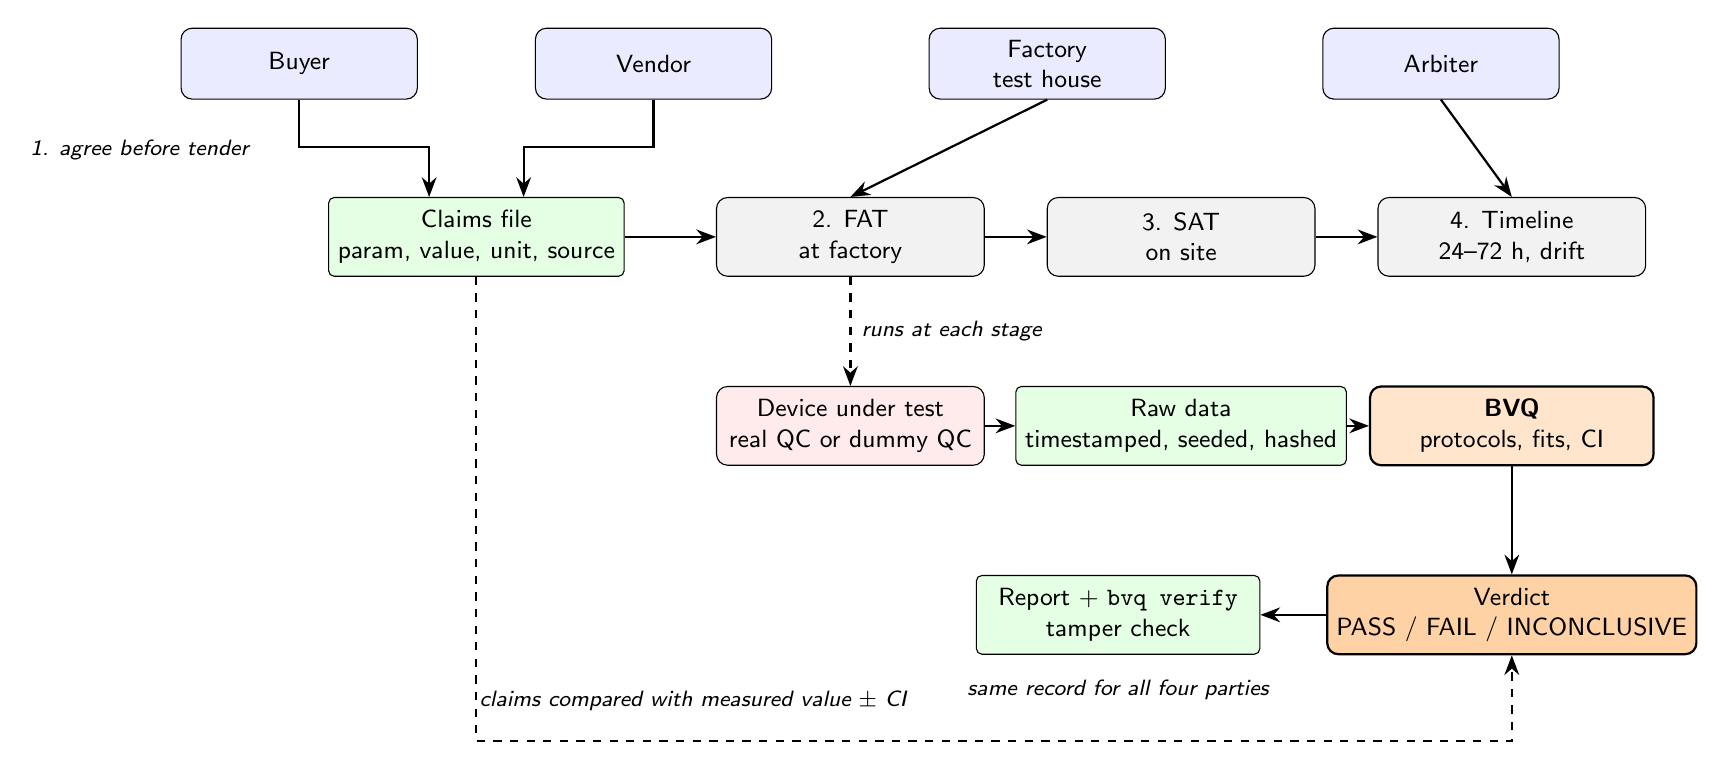
\begin{tikzpicture}[
  font=\sffamily\small,
  actor/.style={draw,rounded corners,fill=blue!8,minimum width=3cm,minimum height=0.9cm,align=center},
  stp/.style={draw,rounded corners,fill=gray!10,minimum width=3.4cm,minimum height=1.0cm,align=center},
  tool/.style={draw,thick,rounded corners,fill=orange!20,minimum width=3.6cm,minimum height=1.0cm,align=center},
  data/.style={draw,rounded corners=2pt,fill=green!10,minimum width=3.6cm,minimum height=1.0cm,align=center},
  arr/.style={-{Stealth[length=2.5mm]},thick},
  lab/.style={font=\sffamily\footnotesize\itshape,inner sep=1pt}
]
% row 1: people
\node[actor] (buyer)  at (0,7)    {Buyer};
\node[actor] (vendor) at (4.5,7)  {Vendor};
\node[actor] (fact)   at (9.5,7)  {Factory\\test house};
\node[actor] (arb)    at (14.5,7) {Arbiter};
% row 2: stages
\node[data] (claims) at (2.25,4.8) {Claims file\\param, value, unit, source};
\node[stp]  (fat) at (7,4.8)    {2. FAT\\at factory};
\node[stp]  (sat) at (11.2,4.8) {3. SAT\\on site};
\node[stp]  (ops) at (15.4,4.8) {4. Timeline\\24--72 h, drift};
\draw[arr] (buyer.south) -- ++(0,-0.6) -| ($(claims.north)+(-0.6,0)$);
\draw[arr] (vendor.south) -- ++(0,-0.6) -| ($(claims.north)+(0.6,0)$);
\node[lab,anchor=east] at (-0.6,5.9) {1. agree before tender};
\draw[arr] (claims) -- (fat);
\draw[arr] (fat) -- (sat);
\draw[arr] (sat) -- (ops);
\draw[arr] (fact.south) -- (fat.north);
\draw[arr] (arb.south) -- (ops.north);
% row 3: device -> raw -> BVQ
\node[stp,fill=red!8] (dev) at (7,2.4)  {Device under test\\real QC or dummy QC};
\node[data] (raw) at (11.2,2.4) {Raw data\\timestamped, seeded, hashed};
\node[tool] (eng) at (15.4,2.4) {\textbf{BVQ}\\protocols, fits, CI};
\draw[arr] (dev) -- (raw);
\draw[arr] (raw) -- (eng);
\draw[arr,dashed] (fat.south) -- (dev.north);
\node[lab,anchor=west] at (7.1,3.6) {runs at each stage};
% row 4: verdict + report
\node[tool,fill=orange!35] (verd) at (15.4,0) {Verdict\\PASS / FAIL / INCONCLUSIVE};
\node[data] (rep) at (10.4,0) {Report + \texttt{bvq verify}\\tamper check};
\draw[arr] (eng) -- (verd);
\draw[arr] (verd) -- (rep);
% claims into verdict
\draw[arr,dashed] (claims.south) -- ++(0,-5.9) -| ($(verd.south)+(0,-0.0)$);
\node[lab] at (5,-1.1) {claims compared with measured value $\pm$ CI};
\node[lab] at (10.4,-0.95) {same record for all four parties};
\end{tikzpicture}
\end{document}
